\documentclass[12pt]{article}
\usepackage{graphicx}
\usepackage{subcaption}
\usepackage{hyperref}
\usepackage{float}
\usepackage[margin=1in]{geometry}

\title{CarND Vehicle Detection Project Writeup}
\author{Tiffany Huang}
\date{\today}

\begin{document}
\maketitle


\section{Vehicle Detection Project}
This project consists of the following steps/tasks:
\begin{itemize}
\item {Perform a Histogram of Oriented Gradients (HOG) feature extraction on a labeled training set of images and train a Linear SVM classifier.}
\item {Optionally, apply a color transform and append binned color features, as well as histograms of color, to the HOG feature vector.}
\item {Normalize the features and randomize a selection for training and testing.}
\item {Implement a sliding-window technique and use the trained classifier to search for vehicles in images.}
\item {Run the pipeline on a video stream and create a heat map of recurring detections frame by frame to reject outliers and follow detected vehicles.}
\item {Estimate a bounding box for vehicles detected.}
\end{itemize}
My project code can be found here: \url{https://github.com/tahuang/Vehicle_Detection}. Next, I will consider each of the rubric points individually and describe how I addressed each point in my implementation.

\section{Histogram of Oriented Gradients (HOG)}

\subsection{HOG Feature Extraction}
The code for extracting HOG features from the training images is in section 1 of \newline
\texttt{vehicle\_detection.ipynb} in the \texttt{get\_hog\_features} and \texttt{extract\_features} functions. I started by reading in all the \texttt{vehicle} and \texttt{non-vehicle} images. I then used \texttt{skimage.hog()} to extract the HOG features. Here is an example of one of each class:
\begin{figure}[!h]
\centering
\begin{subfigure}{0.495\textwidth}
\centering
\includegraphics[scale=2]{../vehicles/GTI_Far/image0007.png}
\caption{Car}
\end{subfigure}
\begin{subfigure}{0.495\textwidth}
\centering
\includegraphics[scale=2]{../non-vehicles/GTI/image8.png}
\caption{Not a Car}
\end{subfigure}
\end{figure}

\subsection{HOG Parameter Selection}
I settled on my final choice of HOG parameters of \texttt{orient=9}, \texttt{pix\_per\_cell=8}, and \newline
\texttt{cells\_per\_block=(2,2)} by trying various combinations of parameters and seeing which ones resulted in the highest score when testing the Linear SVM classifier. This set of parameters had the best test performance of 0.9924. Here is an example of what the HOG features look like with these parameters for a car image using the YCrCb color space:
\begin{figure}[!h]
\centering
\begin{subfigure}{0.32\textwidth}
\centering
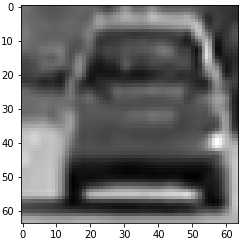
\includegraphics[scale=0.5]{car_ycrcb_ch1.png}
\caption{Car YCrCb Ch 1}
\end{subfigure}
\begin{subfigure}{0.32\textwidth}
\centering
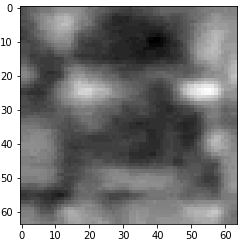
\includegraphics[scale=0.5]{car_ycrcb_ch2.png}
\caption{Car YCrCb Ch 2}
\end{subfigure}
\begin{subfigure}{0.32\textwidth}
\centering
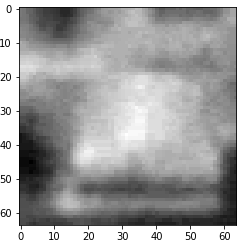
\includegraphics[scale=0.5]{car_ycrcb_ch3.png}
\caption{Car YCrCb Ch 3}
\end{subfigure}
\begin{subfigure}{0.32\textwidth}
\centering
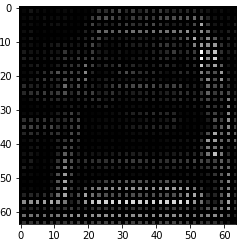
\includegraphics[scale=0.5]{car_hog_ch1.png}
\caption{Car HOG Ch 1}
\end{subfigure}
\begin{subfigure}{0.32\textwidth}
\centering
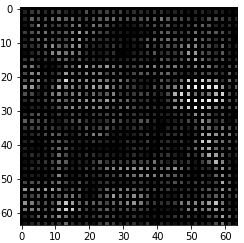
\includegraphics[scale=0.5]{car_hog_ch2.png}
\caption{Car HOG Ch 2}
\end{subfigure}
\begin{subfigure}{0.32\textwidth}
\centering
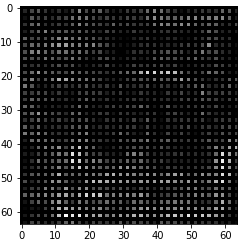
\includegraphics[scale=0.5]{car_hog_ch3.png}
\caption{Car HOG Ch 3}
\end{subfigure}
\end{figure}

These are the HOG features for a non-vehicle image:
\begin{figure}[!h]
\centering
\begin{subfigure}{0.32\textwidth}
\centering
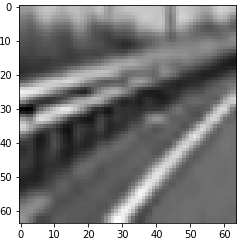
\includegraphics[scale=0.5]{non_car_ycrcb_ch1.png}
\caption{Non-Car YCrCb Ch 1}
\end{subfigure}
\begin{subfigure}{0.32\textwidth}
\centering
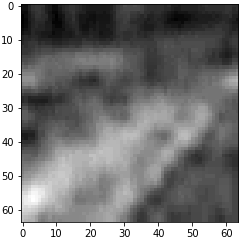
\includegraphics[scale=0.5]{non_car_ycrcb_ch2.png}
\caption{Non-Car YCrCb Ch 2}
\end{subfigure}
\begin{subfigure}{0.32\textwidth}
\centering
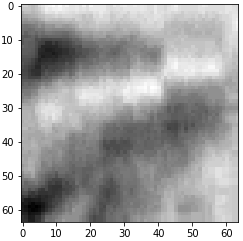
\includegraphics[scale=0.5]{non_car_ycrcb_ch3.png}
\caption{Non-Car YCrCb Ch 3}
\end{subfigure}
\begin{subfigure}{0.32\textwidth}
\centering
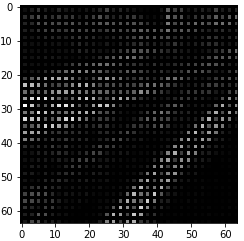
\includegraphics[scale=0.5]{non_car_hog_ch1.png}
\caption{Non-Car HOG Ch 1}
\end{subfigure}
\begin{subfigure}{0.32\textwidth}
\centering
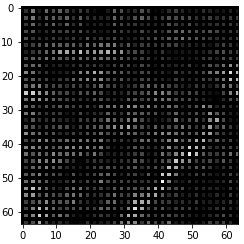
\includegraphics[scale=0.5]{non_car_hog_ch2.png}
\caption{Non-Car HOG Ch 2}
\end{subfigure}
\begin{subfigure}{0.32\textwidth}
\centering
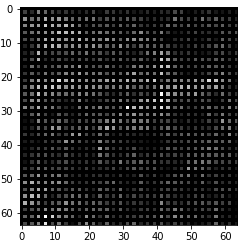
\includegraphics[scale=0.5]{non_car_hog_ch3.png}
\caption{Non-Car HOG Ch 3}
\end{subfigure}
\end{figure}

\subsection{Training a Classifier}
I trained a Linear SVM classifier in section 2 of \texttt{vehicle\_detection.ipynb} where I used spatial color features, color histogram features, and HOG features. I randomly split the training data into training and test sets, then normalized all the data by fitting a \texttt{StandardScaler} to the training data split. I then did a parameter search on the classifier to find the best \texttt{C} value and tested the classifier on the split off test set. The best C value was 0.1 and the classifier test accuracy was 0.9924. Below is an example of the spatial color features and the color histogram features:
\begin{figure}[!h]
\centering
\begin{subfigure}{0.495\textwidth}
\centering
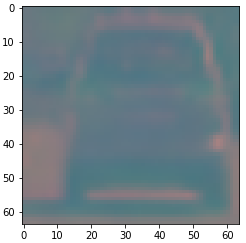
\includegraphics[scale=0.5]{car_ycrcb.png}
\caption{Car YCrCb Image}
\end{subfigure}
\begin{subfigure}{0.495\textwidth}
\centering
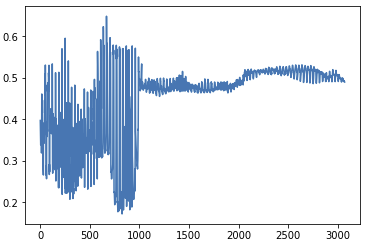
\includegraphics[scale=0.5]{car_spatial.png}
\caption{Car YCrCb Spatial Color Features}
\end{subfigure}
\begin{subfigure}{0.99\textwidth}
\centering
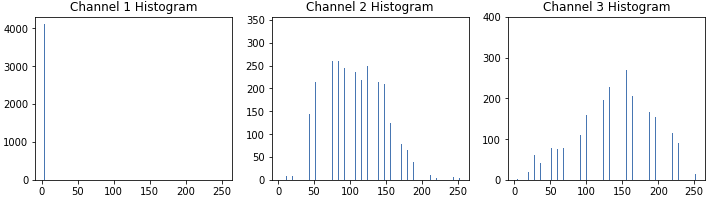
\includegraphics[scale=0.6]{car_color_hist.png}
\caption{Car YCrCb Color Histogram}
\end{subfigure}
\end{figure}

\begin{figure}[!h]
\centering
\begin{subfigure}{0.495\textwidth}
\centering
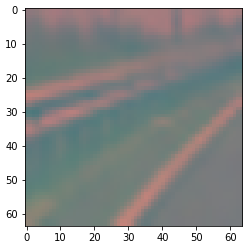
\includegraphics[scale=0.5]{non_car_ycrcb.png}
\caption{Non-Car YCrCb Image}
\end{subfigure}
\begin{subfigure}{0.495\textwidth}
\centering
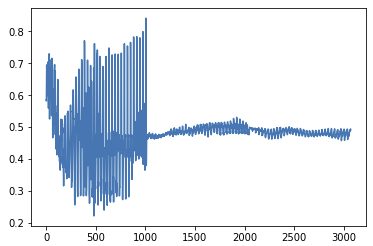
\includegraphics[scale=0.5]{non_car_spatial.png}
\caption{Non-Car Spatial Color Features}
\end{subfigure}
\begin{subfigure}{0.99\textwidth}
\centering
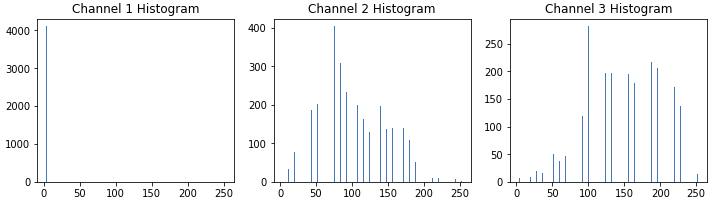
\includegraphics[scale=0.6]{non_car_color_hist.png}
\caption{Non-Car Color Histogram}
\end{subfigure}
\end{figure}

\vspace{30cm}
\section{Sliding Window Search}
\subsection{Sliding Window}
I implemented the sliding window search in section 3 of \texttt{vehicle\_detection.ipynb}. I tested a couple different scales and window overlaps and picked the parameters that produced the best performance on the test images. The scales I used were 1, 1.5, and 2 and the window search was 8 pixels per cell and 8 cells per window with a cell step size of 2.

\subsection{Working Pipeline}
For my pipeline, I used the YCrCb color space, 3-channel HOG features, spatially binned color features, and color histogram features to detect vehicles. I optimized the classifier by trying different parameter sets and choosing the best one. I also added the spatial and histogram features in addition to the HOG features to increase robustness. Here are some example images of the pipeline working:
\begin{figure}[!h]
\centering
\begin{subfigure}{0.495\textwidth}
\centering
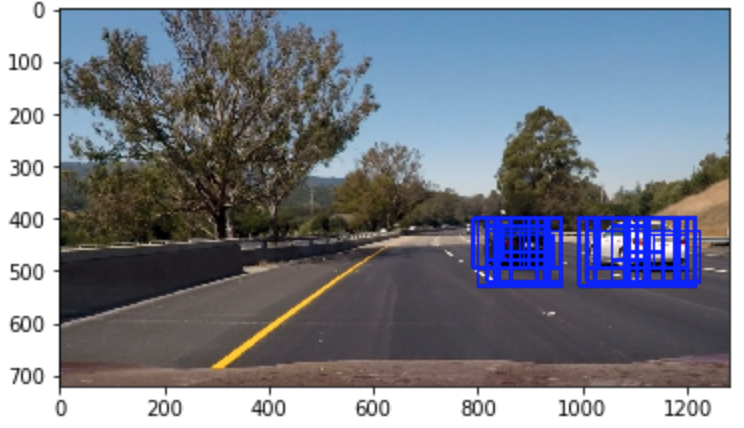
\includegraphics[scale=0.6]{example1.png}
\caption{Example 1}
\end{subfigure}
\begin{subfigure}{0.495\textwidth}
\centering
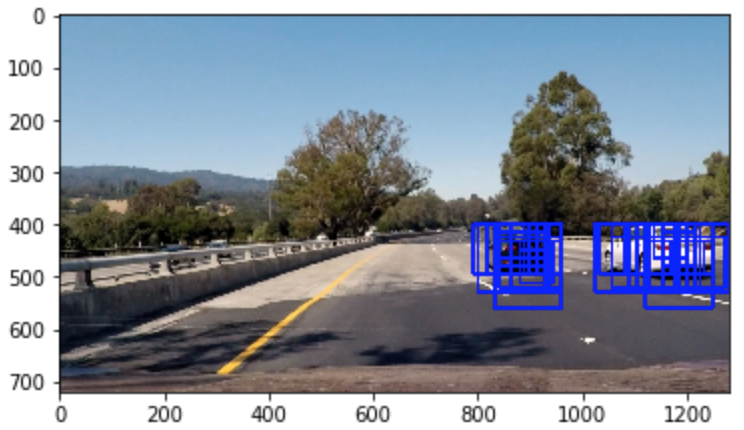
\includegraphics[scale=0.6]{example2.png}
\caption{Example 2}
\end{subfigure}
\begin{subfigure}{0.495\textwidth}
\centering
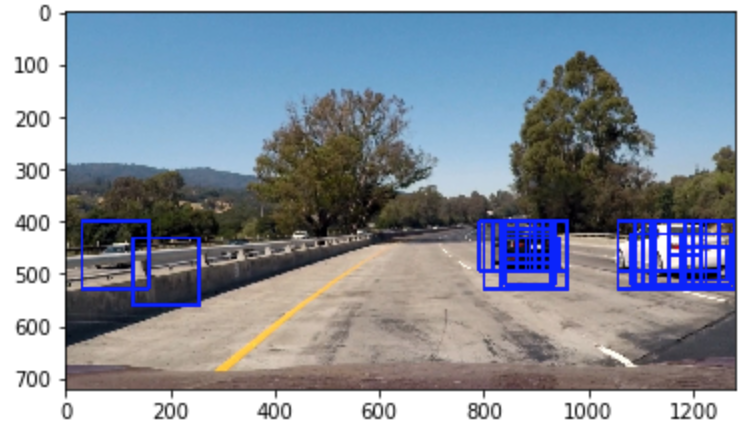
\includegraphics[scale=0.6]{example3.png}
\caption{Example 3}
\end{subfigure}
\begin{subfigure}{0.495\textwidth}
\centering
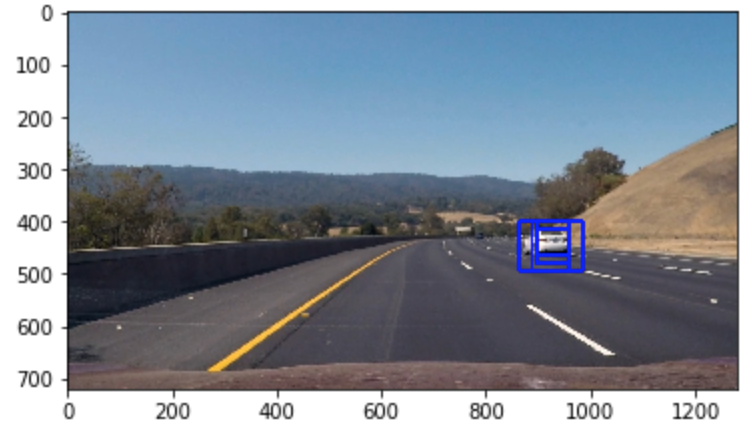
\includegraphics[scale=0.6]{example4.png}
\caption{Example 4}
\end{subfigure}
\end{figure}

\section{Video Implementation}
\subsection{Video}
My video can be found in the \texttt{vehicle\_detection\_project\_video.mp4} file. 

\subsection{False Positives}
To filter out false positives and combine overlapping bounding boxes, I created a heatmap for detections and thresholded the heatmap to throw out weak detections ($\le 2$ detections). The implementation of the heatmap functions can be found in section 4 of \texttt{vehicle\_detection.ipynb}. I then used \texttt{scipy.ndimage.measurements.label()} to identify individual blobs in the heatmap. Once the vehicle blobs were detected, I drew bounding boxes over the blobs. Here is an example of the bounding boxes found, the heatmap generated, the labeled heatmap, and the final filtered result.
\begin{figure}[!h]
\centering
\begin{subfigure}{0.495\textwidth}
\centering
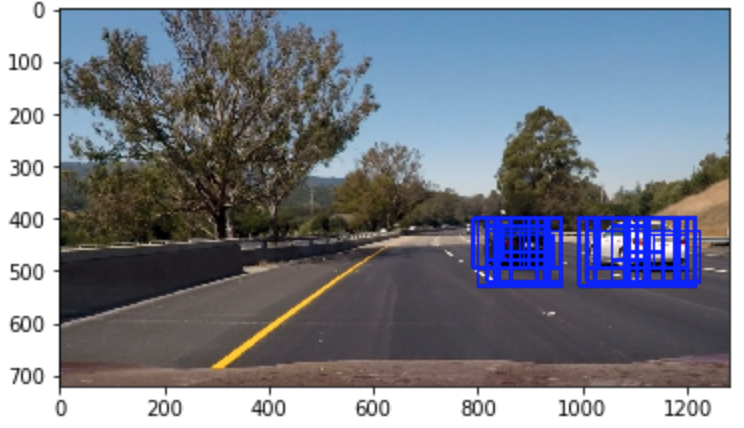
\includegraphics[scale=0.6]{example1.png}
\caption{Non-filtered Bounding Boxes}
\end{subfigure}
\begin{subfigure}{0.495\textwidth}
\centering
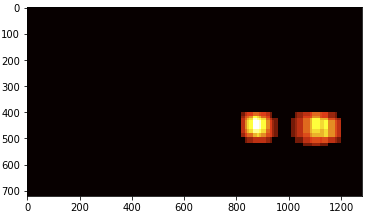
\includegraphics[scale=0.6]{heatmap_ex1.png}
\caption{Heatmap}
\end{subfigure}
\begin{subfigure}{0.495\textwidth}
\centering
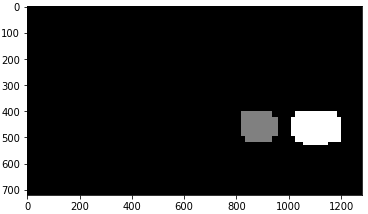
\includegraphics[scale=0.6]{labels_ex1.png}
\caption{Labeled Blobs}
\end{subfigure}
\begin{subfigure}{0.495\textwidth}
\centering
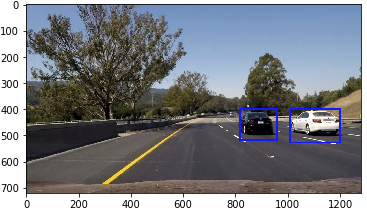
\includegraphics[scale=0.6]{filtered_ex1.png}
\caption{Filtered Result}
\end{subfigure}
\end{figure}

\section{Discussion}
The approach I used was to convert the images into the YCrCb color space, extract spatially binned color features, color histogram features, and HOG features, and use a Linear SVM classifier to detect vehicles. I believe the YCrCb color space worked out well because the luminance (Y) component captures the idea that cars are metallic and usually brighter than the road surface and surrounding objects. The Cr and Cb components capture the blueish and reddish tints that many dark-colored cars contain. The HOG features really capture the shape of the car and help to distinguish it from similarly colored objects in the background. The pipeline might fail if we see cars that were not in our training set. For instance, if there was a dump truck on the road that we had never seen before in the training set, it is possible we would not be able to identify it if the HOG features were quite different. The pipeline also fails for cars that are far away or occluded because it is no longer possible to distinguish their distinctive gradient features. The pipeline might also fail if we see a car from a different angle than we have seen before in our training data because the newly angled car could have different spatial color and HOG features that do not match other cars in the training set. To make the classifier more robust, we could augment the training data with all types of cars and angles of cars. If we did this, we would also have to add more non-car examples so that the training data is not biased towards a vehicle classification.

\end{document}
